
% 物料
    \section {物料管理}

-

    \begin{center}
        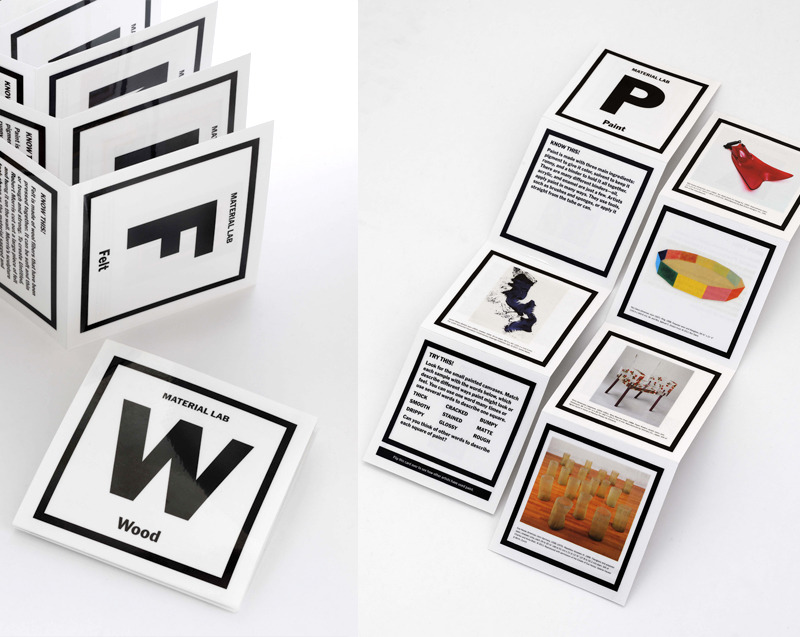
\includegraphics[scale=.3] {cards.jpg}
    \end{center}

    物料管理是将管理功能导入企业产销活动过程中,希望以经济有效的方法,及时取得供应组织内部所需之各种活动。

    物料管理概念的采用起源于第二次世界大战中航空工业出现的难题。生产飞机需要大量单个部件,很多部件都非常复杂,而且必须符合严格的质量标准,这些部件又从地域分布广泛的成千上万家供应商那里采购,很多部件对最终产品的整体功能至关重要。

    物料管理概念的采用起源于第二次世界大战中航空工业出现的难题。

    生产飞机需要大量单个部件,很多部件都非常复杂,而且必须符合严格的质量标准,这些部件又从地域分布广泛的成千上万家供应商那里采购,很多部件对最终产品的整体功能至关重要。物料管理就是从整个公司的角度来解决物料问题,包括协调不同供应商之间的协作,使不同物料之间的配合性和性能表现符合设计要求;提供不同供应商之间以及供应商与公司各部门之间交流的平台;控制物料流动率。计算机被引入企业后,更进一步为实行物料管理创造了有利条件,物料管理的作用发挥到了极致。

\subsection {物料的定义和特性}

    组成产品结构的最小单元是物料。在英文里“物料”有多种叫法,当我们说“物料需求计划” 时,“物料” 在英文里对应的是 materia1。 当我们说 “物料编码” 时,英文里的物料是 item 或 part。在一些国产 ERP 软件里,也有用 “物项”、 “物品”、 “物件”的,很不统一。我们顺着“物料需求计划”的词义,采用“物料”的叫法。

    这里所说的物料,指的是:凡是要列入计划、控制库存、控制成本的物件的统称。包括所有的原材料、配套件、毛坯、半成品、联产品、 副产品、回收品、需要处理的废品、包装材料、标签、说明书、技术文件、合格证、产成品、工艺装备、甚至可以是不能存储的某些能源等。换句话说,物料是计划的对象,库存的对象和成本的对象。

    从管理学角度看,物料的管理特性(家乡材料有物理性能和化学性能一样)主要是3个方面。

    \begin{enumerate}
        \item 相关性

        从供需链的概念出发,任何一种物料都是由于某种需求而存在的,没有需求的物料,就没有产生或保存的必要。一种物料的消耗量受另一种物料的需求量制约,如购买原材料是为了加工零件,而生产零件又是为了装配产品; MRP 理念的基本出发点就是平衡供需关系。从大范围来讲,一个企业的原料是另一个企业的产品= 一一个企业的产品,又是另一个企业的原料。

        只有当市场有需求时,企业生产的产品才有价值。这种相关需求不但有品种规格、性能、质量和数量的要求,而且有时间和空间 (需用时间和地点) 的要求。

        \item 流动性

        既然任何物料都是由于某种需要而存在,它就必然处于经常流动的状态,而不应当在某个地点长期滞留。物料的相关性必然形成物料的流动性,不流动的物料只能是一种没有需求的积压浪费。通过物料的流动性来检查物料在相关性上存在的问题,是物料管理或物流管理的一项重要内容。

        \item 价值

        物料是有价值的。库存或存货是流动资产,要占用资金; 而资金又是有时间价值的,使用了资金就应体现资金成本,要产生利润。因此,不仅要把库存物料看成是一种资产,还要看到它也是一种 "负债”(尤其是超储物料); 它占用了企业本来可以用来在其他方面获取利润的资金 应当计算机会成本。产品研发人员需要知道每个零部件的价值,从设计源头把住成本关,这也是价值工程学要做的分析工作。

    \end{enumerate}

    只有理解物料的这些管理特性 才能应用好 ERP 系统,做好计划管理、物料管理。

\subsection { 物料管理的目标}

    \begin{enumerate}
        \item  物料规格标准化,减少物料种类,有效管理物料规格的新增与变更。
        \item  适时供应生产所需之物料,避免停工待料。
        \item  适当管制采购价格,降低物料成本。
        \item  确保来料品质良好,并适当的管制供货商。
        \item  有效率的收发物料,提高工作人员之效率,避免呆料、废料之产生。
        \item  掌握物料适当的存量,减少资金的积压。
        \item  可考核物料管理之绩效。
        \item  仓储空间充分的利用。
    \end{enumerate}

\subsection { 物料的分类}

    \subsubsection {(一)功用}

    将材料分为主要材料与辅助材料。主要材料是构成制成品最主要之部份,而辅助材料多半在配合主要材料之加工而附属于制品上。

    \subsubsection {(二)型态}

    将材料分为素材与成型材。素材者仍需加工之材料,它又分为料材与粗型材。成型材为已加工之材料,它又分为配件、零件、组合件。

    \subsubsection {(三)成本管制}

    将材料分为直接材料与间接材料。直接材料使直接供作制品制造之材料,其消耗与产品之产量成正比,如铸件之于马达。间接材料是间接帮助制品之材料,其消耗不一定与产品之产量成正比,辅助材料有时亦包括于间接材料。

    \subsubsection {(四)调度方法}

    将材料分为公司外部调度的第一次材料与公司内部调度的第二次材料。公司外部调度的第一次材料系指公司内购、外购之材料与外加工之材料。第二次材料系指规模较大的公司内部部门很多,由一个部门之材料调度至另一部门。

    \subsubsection {(五)准备方法}

    将材料分为常备材料和非常常备材料。常备材料为利用存货管制的原理,定时购买一定数量的材料,存备这些材料以供生产之需。有些特殊材料不能事先购买存备,必须是生产计划而随时决定购买之材料,是为非常备材料。

\subsection { 物料的特性}

    首先是物料的相关性,任何物料总是由于有某种需求而存在;没有需求的物料就没有存在的必要。

    其次是物料的流动性,既然有需求,物料总是不断从供方向需方流动;物料的相关性决定了物料的流动性。

    物料是有价值的,一方面它占用资金,为了加速资金周转,就要加快物料流动;而另一方面,在物料形态变化和流动的过程中,要用创新竞争(不仅是削价竞争),提高物料的技术含量和附加值,用最小的成本、最短的周期、最优的服务,向客户提供最满意的价值并为企业自身带来相应的利润。这也是增值链(value-added chain)含义之所在。 三种特性相互作用、互相影响。理解物料的管理特性有助于理解物料需求管理的特点。

    在市场竞争日益激烈的环境下,产品生命周期越来越短,品种越来越多;客户对交货期的要求越来越短;同时,企业对库存的控制也因为成本的压力而变得越来越严格。怎样才能有效地解决这一矛盾,是摆在企业管理者面前的难题。本课程采集了大量不同行业和不同生产组织方式的企业物流模型,结合企业内部供应链管理研究的最新成果,理论结合实际,全方位演绎企业物流管理的真谛,帮助企业建立供应链管理的新模式。

\subsection { 物料管理的原则}

    通常意义上,物料管理部门应保证物料供应适时、适质、适量、适价、适地,这就是物料管理的5R原则,是对任何公司均适用且实用的原则,也易于理解和接受,下面分别进行阐述:

    \begin{enumerate}
    \item  适时:即要求供应商在规定的时间准时交货,防止交货延迟和提前交货。

    供应商交货延迟会增加成本,主要表现在:
        \begin{enumerate}
            \item  由于物料延迟,车间工序发生空等或耽搁,打击员工士气,导致效率降低、浪费生产时间;
            \item  为恢复正常生产计划,车间需要加班或在法定假期出勤,导致工时费用增加。
        \end{enumerate}

    因此应尽早发现有可能的交货延迟,从而防止其发生;同时也应该控制无理由的提前交货,提前交货同样会增加成本,主要原因为:
        \begin{enumerate}
            \item  交货提前造成库存加大,库存维持费用提高;
            \item  占用大量流动资金,导致公司资金运用效率恶化。
        \end{enumerate}

    \item  适质:即供应商送来的物料和仓库发到生产现场的物料,质量应是适当的,符合技术要求的。

    保证物料适质的方法如下:
        \begin{enumerate}
            \item  公司应与供应商签订质量保证协议;
            \item  设立来料检查职能,对物料的质量做确认和控制;
            \item  必要时,派检验人员驻供应商工厂(一般针对长期合作的稳定的供应商采用,且下给该供应商的订单达到其产能的30\%以上);同时不应将某个检验人员长期派往一个供应商处,以防其间关系发生变化;
            \item  必要时或定期对供应商质量体系进行审查;
            \item  定期对供应商进行评比,促进供应商之间形成良性有效的竞争机制;
            \item  对低价位、中低质量水平的供应商制订质量扶持计划;
            \item  必要时,邀请第三方权威机构做质量验证。
        \end{enumerate}

    \item  适量:采购物料的数量应是适当的,即对买方来说是经济的订货数量,对卖方而言为经济的受订数量。

    确定适当的订货数量应考虑以下因素:
        \begin{enumerate}
            \item  价格随采订货数量大小而变化的幅度,一般来说,订货数量越大,价格越低;
            \item  订货次数和采购费用;
            \item  库存维持费用和库存投资的利息。
        \end{enumerate}

    \item  适价:采购价格的高低直接关系到最终产品或服务价格的高低,在确保满足其它条件的情况下力争最低的采购价格是采购人员最重要的工作。

    采购部门的职能包括标准化组件,发展供应商,发展替代用品,评估和分析供应商的行为。为了达到这一目标,采购部门应该在以下领域拥有决策权:
        \begin{enumerate}
            \item  选择和确定供应商;
            \item  使用任何一种合适的定价方法;
            \item  对物料提出替代品;

            采购部门通常能够提供出目前在用物料的替代品,而且它也有责任提请使用者和申请采购者关注这些替代品。当然,是否接受这些替代品要由使用者/设计人员最终作出决定;
            \item  与潜在的供应商保持联系。

            采购部门必须和潜在的供应商保持联系。如果使用者直接与供应商联系,而采购部门又对此一无所知的话,将会产生“后门销售”,即潜在的供应商通过影响使用者对物料规格方面的要求成为唯一的供应商,或是申请采购者私下给供应商一些许诺,从而使采购部门不能以最低的价格签订理想的合同。如果供应商的技术人员需要和公司技术人员或生产人员直接交换意见,采购部门应该负责安排会谈并对谈判结果进行审核。
        \end{enumerate}

    \item  适地:物料原产地的地点应适当,与使用地的距离越近越好。距离太远,运输成本大,无疑会影响价格,同时沟通协调、处理问题很不方便,容易造成交货延迟。

    高科技行业对产品质量普遍要求很高,致使各企业对生产制造环节管理越来越精细,但对产品的物料管理环节却依旧保持比较粗放的管理风格,使物料在很大程度上占用了企业资金,无形中导致成本增长,利润下降。物料管理是企业内部物流各个环节的交叉点,衔接采购与生产、生产与销售等重要环节,关乎企业成本与利润的生命线,不仅如此,物料管理还是物资流转的重要枢纽,甚至关系到一个企业存亡。曾听过一个关于爱多的例子,据说爱多在破产之际,库存物料的金额高达上亿元,可就是这么多的物料中,居然无法组装出一个完整的DVD成品,在惊叹之余,更激起人们对于制造企业物料呆滞及不合理管库问题的思考。

    有资料表明,企业的存货资金平均占用流动资产总额的40\%-50\%,而高科技制造企业的库存比例则远高于此。“物料存在两套或多套编码”、“物料混乱堆积在仓库各个角落”,成为许多制造企业仓库的真实写照。就曾有人套用中央电视台著名的广告语“心有多大,舞台就有多大”放在制造型企业身上,演绎成“仓库有多大,库存就有多高”,形象地表述了普遍存在于制造型企业内部库存管理问题的顽疾。

    \end{enumerate}

\subsection { 物料管理的职能机构}

    一个小公司的发展可分为三个阶段:完全整合、职能独立、相关职能的再整合。

    一个公司初创时,几乎所有的工作都是由总经理(通常是公司的所有者)或是组成领导小组的公司主要成员来完成的。

    随着公司的发展和壮大,公司业务量和工作人员逐渐增多,相应的职能逐步独立形成职能部门,例如,采购、仓储、运输、生产计划、库存控制和质量控制等职能都形成了独立的部门,并致力于专门的管理工作,公司业务上的分工也日益专业化。

    各职能部门独立后,各部门之间的沟通机会越来越少,于是部门之间合作的问题经常出现,矛盾一点点加深。最终我们又可以清楚地看到,如果能减少由于沟通和合作而产生的问题,把相互之间有密切联系的职能部门重新加以整合,公司就可以极大程度地受益。

    于是,与物料管理有密切联系的各职能部门被重新整合到一起。

\subsubsection {部门的职能范围}

    一般来说,物料管理部门的职能包括以下方面:

    \begin{itemize}
    \item  物料的计划和控制

        即根据项目主合同交货时间表、车间生产计划和项目技术文件等确定物料需求计划,并根据实际情况和项目技术更改通知等文件随时调整物料需求数量,控制项目材料采购进度和采购数量。

    \item  生产计划

        根据项目主合同交货时间表和材料采购进度编制车间生产计划,并根据实际情况和项目计划随时调整,使车间生产计划与项目主合同交货时间表保持一致。

    \item  采购

    根据车间生产计划对生产所需要的物料进行准确的分析,并制订完整的采购计划;严格地控制供应商的交货期和交货数量;

    \item  物料和采购的研究

        收集、分类和分析必要的数据以寻找替代材料;对主要外购材料的价格趋势进行预测;对供应商成本和能力进行分析;开发新的、更为有效的数据处理方法,从而使物料系统更加高效地运转。

    \item  来料质量控制

        即对供应商的交货及时进行来料检查,及时发现来料的质量问题以便于供应商有足够时间处理或补发产品,保证车间及时得到物料供应,保证发送到车间现场的物料全部是合格产品。

    \item  物料收发

        负责物料的实际接收处理、验明、通知质量作来料质量检验,以及将物料向使用地点和仓储地点发送。

    \item  仓储

        对接收入库的物料以正确的方式进行保管、储存,对储存过程中可能变质或腐蚀的物料,应按一定的防腐蚀和变质的方法进行清洗、防护、特殊包装和存放。

    \item  库存控制

        定期检查物料库存状况,加强物料进出库管理;随时掌握库存变化情况,发现任何异常(包括呆滞料,库存积压或0库存)情况,及时向采购通报。

    \end{itemize}

    当然,并不是所有公司的物料管理部门都包括上述所有职能。根据公司规模大小,公司业务性质不同以及公司不同发展阶段,物料管理部门的职能也不尽相同。

    通过上述文字描述,可知与物料有密切联系的各职能部门被重新整合到一起,这种整合就是物料管理理论的基础,所以,物料管理较仓库管理的范围更为广泛,其中也包括仓库管理。


% 简介
    \section {库存管理}

-

    \begin{center}
        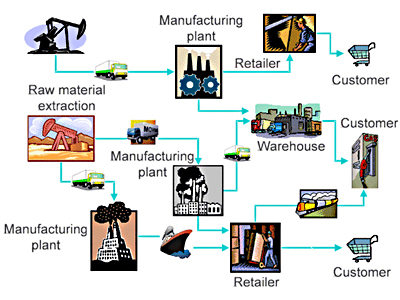
\includegraphics[scale=1.5] {factory.jpg}
    \end{center}

    库存是企业组织中存储的各种物品与资源的总和,是企业在生产和物流渠道中各仓库堆积的原材料、供给品、零部件、半成品和成品等。库存是企业进行正常生产经营活动所必须具备的条件,在企业生产经营过程中,库存能够实现企业的规模经济,满足供求平衡,预防需求和订货周期的不确定性。

    库存管理的宗旨和目标是在保证供应的前提下尽可能的降低成本。库存管理的核心问题是库存控制。库存控制就是确定合理的订货时间和数量,用最少的费用去满足生产和经营的需要。并借以获得最大的经济效益,随着企业走向市场。企业为充分发挥资金的效用,取得较好的经济效益,对库存控制越来越重视。

\subsubsection { 库存对企业的影响}

    如今,企业对库存管理越来越重视,无论它是制造商、分销商、批发商、零售商,或是其他类型的行业企业。因为库存资产在企业总资产额中所占比率相当可观,降低库存是实质性地减少流动资金需求的最快方式之一。库存周转把资产转变为利润,库存周转越快,收益率越好。诸如资产回报率以及其它一些资金使用效率方面的评价越来越普遍地影响着组织。在公司中,库存起着如下五个作用:

    \begin{enumerate}
        \item  使公司有可能达到规模经济;
        \item  平衡供求;
        \item  使制造专业化成为可能;
        \item  保护公司少受需求和订货周期的影响;
        \item  在分配渠道间起缓冲器作用。
    \end{enumerate}

\subsubsection { 库存对物流的影响}

    从某种意义上讲,仓储管理在物流管理中占据着核心的地位。这是因为库存总是出现在物流各环节的接合部,例如采购与生产之间,生产的初加工与精加工之间,生产与销售之间,批发与零售之间,不同运输方式转换之间等等。仓储是物流各环节之间存在不均衡性的表现,库存也正是解决这种不均衡性的手段。仓储环节集中了上下游流程整合的所有矛盾,库存管理就是在实现物流流程的整合。如果借用运筹学的语言来描述仓储管理在物流中的地位,可以说就是在运输条件为约束力的情况下,寻求最优库存(包括布局)方案作为控制手段,使得物流达到总成本最低的目标。在许多具体的案例中,物流的整合、优化实际上归结为仓储的方案设计与运行控制。

\subsection {库存控制}

    库存信息对财务的资产负债表和损益表有直接的关系。 库存是可以交换和销售的流动资产,一般约占企业资产的 20\%~60\%。在损益表中以销售产品成本的形式出现,它是说明企业收益的重要因素。库存反映了企业财务状况的好坏。因此,库存管理非常重要,不能仅仅看成是一个记好库存台账的问题。

    库存管理因计划与控制的层次(独立需求件、相关需求件)、物料对象(产品、在制品、半成品、原材料、MRO)、物料的 ABC 分类、 供需链上的地位(供应、制造、分销)、物料供应周期的长短而异。在供需链上每一个经济实体之间,都有可能出现库存和运输。

    在 APICS 词汇中 “库存 (inventory)” 一词的定义是: “以支持生产、维护、操作和客户服务为目的而存储的各种物料;包括原材料和在制品、维修件和生产消耗品、成品和备件等”。

    因此,库存管理主要是: “与库存物料的计划与控制有关的业务”,目的是支持生产运作。注意,不要把它同仓库管理系统〈WMS〉混淆起来。仓库管理系统主要针对仓库或库房的布置、物料运输和搬运、存储自动化等的管理。两者的概念是不同的。

    库存是计划的结果,又是支持计划实现的先决条件。因此,库存管理的首要任务是根据产品计划的要求来控制库存。传统管理习惯把库存管理理解为仅仅是物料的 “入库、存储、出库”,也就是库存事务的一部分工作,这是不全面的。库存管理如果不同计划管理结合起来,就不能说明库存物料的品种,数量和存储时间是否合理,即不能说明库存物料在数量上是存多了还是存少了,在时间上是存早了还是存晚了。库存量应当是计划的结果,库存脱离了计划,就谈不上控制。库存管理除了保证库存信息准确,满足客户和市场需求计划外,一项重要任务是控制库存量,加速库存周转,降低成本。换句话说,评价库存管理的标准主要是

    \begin{itemize}
        \item 客户服务水准,既保证生产和销售的需求又控制资金占用;
        \item 库存占用的资金额,控制在企业预算之内;
        \item 库存资金周转次数,超过、保持或接近行业领先水平。
    \end{itemize}

    库存周转次数计算公式\eqref{eq:inventoryCycle}如下:

    \begin{equation} \label{eq:inventoryCycle}
        库存资金周转次数(次)=
            \cfrac{ \displaystyle 产品年销售成本(元)}{ \displaystyle 库存年平均占用资金额(元)}
    \end{equation}

    这里考核的只是库存资金占用,而不是企业全部流动资金。换句话说,只是流动资金中的盘存资产部分,即储备资金、生产资金和成品资金,不包括结算(如应收账款)和货币资金。这样处理,同成本计算采用制造成本法是一致的。它反映丁企业的库存管理水平。在考核企业业绩时,库存资金周转次数是一项重要的指标,说明为了实现某个销售金额需要用于库存的流动资金的金额数。通过实施 ERP,既要增加销售收入,又要提高库存资金周转次数。通俗地说,就是一个钱能顶几个钱用。库存占用资金同销售收入两者之间并不存在必然的线性关系,管理的目标是:既要增加销售收入又要降低库存资金占用。

    库存控制同计划层次对应,也有宏观和微观两个层次。宏观层主要控制会计年度内的库存水准,作为财务预算的依据。控制库存水准的主要参考值是同行业类似企业在类似客户服务水准下的库存周转次数。按照高标准定位的精视应高于同行业的平均库存周转次数。

    微观层主要针对库存事务、盘点及储运等,也就是软件中库存管理的主要功能。日本的JIT哲理,把库存量比作江湖的水量,把水下的礁石比作由于管理不善造成的各种问题,如预测不准、供应不及时、计划不周、能力不足、质量不高、不重视培训、设备保养差等等。库存量大了相当于水位高了,淹没了水下的礁石,看上去有利于通航,但是水下被掩盖了的问题(瞧石)却馗不能暴露出来,也永远手寻不到彻底解决。因此,库存量过大被喻之为 “众弊之源”。就是说,库存量掩盖的管理问题是永远不会自动消除的。如图 \ref{fig:inventoryShip}所示。

    \begin{figure}[h]
        \centering
        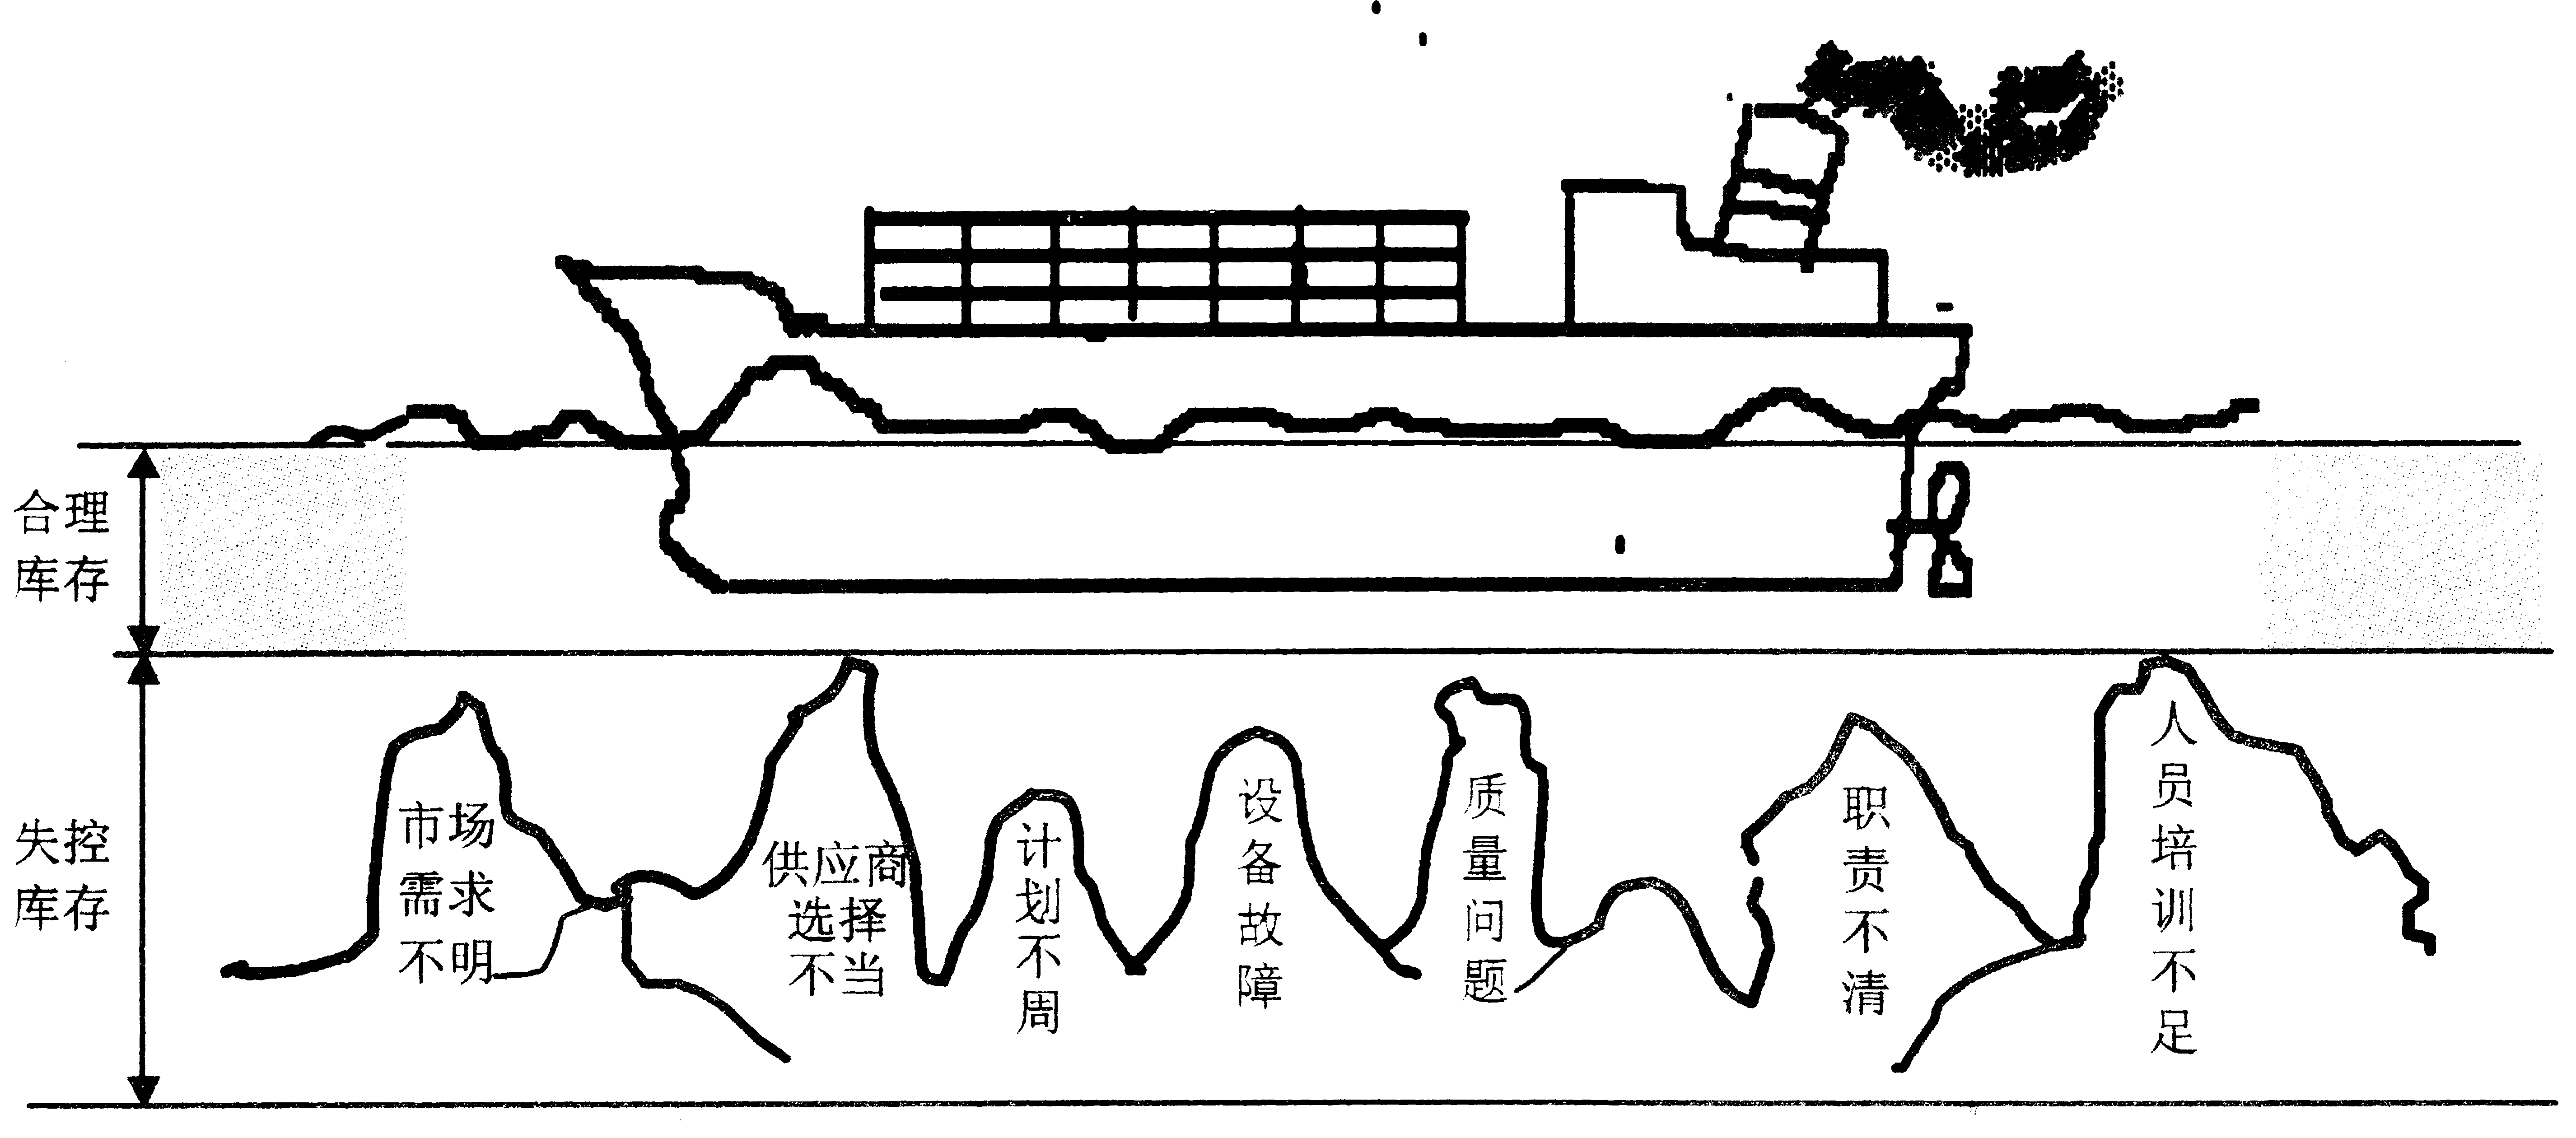
\includegraphics[scale=0.75]{inventoryShip.png}
        \caption{过量库存掩盖管理不善的问题} \label{fig:inventoryShip}
    \end{figure}

    人总是有一些惰性,总是希望工作轻松一点。因此,只有当库存资金占用影响了企业的竞争力或利润时,才会下决心去降低库存。这个要求通常是企业老总提出来的,北京一个汽车厂,平时生产线上储存了 2\~3 天的用量,习以为常,后来老总提出要求降到 10 件,促使员工精心操作,实现了新的目标。真是: “老总不发话,库存降不下”。

    从图 \ref{fig:inventoryShip} 里也可以看出,任何船只都会有一定的吃水量,没有水是不能行船的。这里提出 “合理库存”,而不是 “零库存”。零库存是一种控制库存的哲埋,为的是减少一切无效作业与浪费,要有效地使用各个系统和各种技术。例如: 预测要准,加工周期要短,质量要保证,供应商要可靠等。总之,是追求消除不必要的多余库存,而不是追求 “没有” 库存。一个企业自己可以做到 “零” 库存,但是从供需链管理的角度来看,只是库存转移,或 “嫁祸于人”,把原材料存在供应商的仓库,把产成品存在经销商的仓库。因此,要用整体拥有成本(TCO)全面而系统地权衡。

    控制库存量是物料管理的重要内容,在确定库存量时要注意库存目的和库存费用。

\subsection {库存的目的}

    如果库存没有目的也就没有储存的必要,这督是控制库存时第一个要考虑的问题。库存的目的主要是为了保证生产和销售正常进行,它有 5种常见的基本类型。

    \begin{enumerate.zh}
        \item 安全库存(safety Stock 或 fluctuation inventory)。有时也称最小库存余量(minimum ba1ance)或最低库存。

        企业内外的需求和供给都可能出现偏离计划或预测的情况,会遇到许多不确定因素。为了不中断生产,在计划需求量之外经常保持一定的库存量作为保险储备。安全库存是物料主文件中一项用户设定的参数,当实际库存量低于安全库存量时,系统会自动生成定单建议用户补足安全库存。

        \item 季节性储备(seasona1 stock)或预期储备(anticipation inventory)。

         受季节供应约束的采购件(如农产品)、受季节市场需求约束的产品(如服装、空调机、节日礼品)、或为工厂休假日及因设备计划检修需要事先储备的物料,统称季节性储备或预期储备。 这类库存一股是可以预计的,用销售与运作计划(S\&OP)来规划。

        \item 批量库存(1ot size inventory 或 working stock)。

        受供应、加工、运输、包装或享受折扣优惠等因素的影响。必须按一定的批量生产或采购。由此形成可能超出实际需要的库存称为批量库存。当批量规则是采用固定批量法时,这类库存尤为突出。

        \item 在途库存(transportation inventory 或 pipeline stock)。

        对厂内来讲,在途库存是工序之间因传送、等待、缓冲而形成的在制品库存。对厂外来讲,在途库存是为了保持连续向用户供货或连续满足本厂需求,在运输途中保有一定数量的物料,在分销资源计
    划和流程工业中的管道输送中常出现在途库存。此外,财务与实物对账时,例如,己付款但货物尚未到厂入库,也要用到在途库存来对应“在途材来斗” 账户。

        \item 囤积库存(hedge inventory)。

        针对生产常用物料涨价趋势,储备一定数量,以控制今后成本。由于这样做要积压库存资金,必须分析涨价因素同多付利息之间的关系。如果囤积库存不是生产用的物料,应归入 “不可动用量” 中,不参与需求计算。系统可以按用户规定,把超过设定的 “最长允许存储天数(或货架天数)”,在一个期间内未发生任何事务处理的,或超过规定的 “最大存储量” 的物料显示出来提醒管理人员分析原因并采取措施。

    \end{enumerate.zh}

\subsection {库存的费用}

    控制库存量的第二个要注意的问题是库存费用,确定库存费用要考虑4个因素。

    \begin{enumerate.zh}
        \item 物料价值。

        物料的单位标准成本或计划价格,在物料主文件中记录。

        \item 定货费(acquisition cost或ordering cost)。

        如前所述,“定货” 包括采购和加工两个方面,是指为了获取物料需要支付的费用。如准备定单、洽谈、运输、搬运、验收、办公和管理等费用。定货费同定货批量和次数有关,批量小,定货次数多,定货费就高。定货费或定货成本通常在物料主文件中记录。

        \item 保管费(carrying cost)。

        保管费是指为了保存物料所支付的费用。如利息、折旧、损耗、财产税、保险等。现代管理把占用资金的机会成本(即这笔资金如果没有作为资金占用而是投资在其他方面所能获得的利益),也计入保管费用,机会成本占保管费用的比例往往在40\%以上,照这样计算,保管费可占到库存价值的 20\%\~35\%。保管费通常用占库存价值的百分比来估算,需要在软件的系统参数中设置。以上 3 项数据在经济批量计算中还会用到,各软件会有具体要求。

        \item 短缺损失(cost of stockout)。

        由于物料出现短缺造成停工待料的损失、紧急定货的额外开支。包括加班加点和紧急采购迟未按期交货造成的客户索赔,撤消定货甚至丧失市场等经济损。

    \end{enumerate.zh}

    以上几项费用相互影响,例如,库存量大可能短缺损失加,但保管费高;要降低保管费就要降低批量,但批量小定货次数增加,定货费用增加。控制库存就是要权衡这些费用,使总费用最低,以实现降低成本的目的。

    通常在控制库存时,由企业领导从宏观上提出一个库存水准的要求,在一种紧迫和危机感的压力下,解决各种管理不善的问题,使库存降到看来似乎已不能再降的程度。经过一个时期,运行已经正常,再提出更高的控制库存水准的要求,进一步挖掘潜力,再次降低库存,从而不断降低成本,满足市场竞争的需要。要做到这点 必须要企业领导提出目标,并监督执行。

\subsection {库存事务}

    除了控制库存外,库存管理的日常工作是库存事务处理,库存事务有 4 种类型:

        \begin{enumerate.zh}
            \item 物料存放位置的变化,即物料的移动。例如,从供应商(采购单)到待验区,从待验区到仓库或退货给供应商,从仓库到车间,从车间到检验区或废品库,从发货区到客户(销售合同)等等。

            \item 物料数量的变化。位置的变化会伴随数量的变化。但是,也有存放位置不变,数量却发生变化的情况。例如,盘点后数量的调整等。

            \item 物料价值的变化。在存放位置和数量都未变化的情况下,物料的价值由于质量,过时废弃等原因在金额(标准成本)上的调整。

            \item 物料状态的变化。在下达定单但是尚未付款或到货的情况,在 ERP 系统会把物料处于一种 “定单状态”,而物料到货入库时则处于一种 “实物状态”。
        \end{enumerate.zh}

    以上 4 类处理便于把事务处理同账务处理对应起来,实现物流信息同资金流信息的集成。

    企业应当列出日常经营生产活动中,都有哪些库存事务,并分析这些事务同什么物理位置发生关系,涉及哪些会计科目,借贷关系如何,又涉及哪些定单。在软件中对每一种库存事务都要有代码并明确定义。

    在分析库存事务的同时,要分析相关的业务流程是否合理。就是说,定义库存事务的过程也是发现业务流程存在问题的过程。

    % 中小企业的库存
        \subsection {中小企业的库存管理问题}

    物资储备以保证企业正常的生产和销售。库存是任何企业必不可少的基本要数,但是又占用着经营者的资金。企业要想提高效益,必须有效地控制库存。于是,企业的经营者们想尽一切办法来降低库存,在占有尽量少的资金前提下,最大限度地满足企业的正常生产和经营。甚至有人提出了零库存的概念,但零库存也还是有库存,只是通过类似VMI的方式将库存占用的资金降低趋向为零。对于企业管理层特别是采购供应链管理者而言,两头平衡库存与资金占用量是不可缺少的功课。

    中小企业是我国经济建没的重要力量,目前中国的中小企业占全部企业数的99\%以上、国内生产总值的50\%。但是我国许多中小企业不同程度地存在影响其发展的问题,主要是企业信息化水平不高。为此,在首届中国西部地区对外经济合作暨中小企业信息化论坛上,国家提出要把推进中小企业信息化进程放在企业发展的优先位置,充分利用信息技术,不断提高企业应用水平,提高企业的开发创新能力、经营管理能力和竞争力。然而,中小企业在其信息化的进程中却举步维艰。信息化程度很低,没有通过使用信息系统改变企业的管理模式和决策程序。致使企业对家底摸不清,对市场变化反应不灵。这种特点是由中小企业库存管理的不足引起的。

    这里分析一下目前中小企业中库存管理存在哪些问题,通过分析企业在库存管理方面存在的问题,提出一些解决的思路。并通过调研青岛胶南几家经营企业以及青岛三江源建筑添加剂有限公司获得的数据进行分析说明。

    \subsubsection { 物资储备过高,库存结构不合理。}

    现在很多中小企业还是完全凭经验管理,对所有存货采用统一的库存控制方式。没有对重点存货进行重点管理,是一种较为粗放的库存管理。没有科学规范的方法,只能设置较高的安全库存以应付企业经常面临的预期外需求,而不是根据不同存货的服务水平以及各自提前期来确定。因此,在物资采购过程中就会缺乏科学的预测,也没有先进的库存数据分析系统,采购人员只能靠经验、订单和季节因素来确定目前企业所需的物资,缺乏具体的市场调研和需求调查,造成库存积压。以青岛三江源建筑添加剂有限公司为例:从2009年底财务报表的数据来看,该企业月产量600公吨,年营业额380多万的情况下,现有资金储备160多万元,其中由于长期积压物资占用的资金约为100万,严重影响企业资金流通。

    \subsubsection { 信息化程度不高,信息化进程缓慢。}

    据《中国中小企业信息化发展报告(2007)》显示,目前中小企业信息化存在的主要问题是,仍有相当数量的中小企业对信息化促进企业发展的作用、效果以及政府支持信息化建设的政策措施了解不够。虽然有高达调研数量80\%的中小企业具有接入互联网的能力,但用于业务应用的只占44.2\%,只有9\%的中小企业实施了电子商务,4.8\%的企业应用了管理软件。统计数据表明,目前,在我国1000万家中小企业中,实施信息化的比例还不到10\%,甚至有些企业仍然采用纯手工操作。另外还有一些原因也制约着中小企业信息化的进程。如:决策层缺乏库存控制意识,忽略库存成本;缺乏成熟的专业库存管理软件;研究开发一套信息化管理系统需要大量的资金。实行一套管理系统涉及到整个企业的各部门利益;现有的信息系统的优势可以被廉价的劳动力取代,从业人员素质低下,难以掌握先进管理技术和优化技术,需要占用大培的时间培训等。

    如瑞鑫物流作为胶南一个小有名气的物流公司,其所谓的库存就是几间仓库,货物的堆放混乱,导致配送人员在货物堆中寻找所需的物件。如中联水泥位于胶南的分公司,由于信息化程度不高,对于同一种材料的多次入库和多次领用,很难计算实时库存,经常由于原材料库存数日不清造成采购不及时或过量采购,从而引发缺货损失或库存积压问题。笔者认为:要想构筑先进的物流系统,提高物流管理水平,单靠物流设备和一个简单的软件来管理库存是远远不足的。

    \subsubsection { 信息不能共享,企业自身库存控制失衡。}

    由于信息不能共享,各部门之间的沟通又不及时,生产部门根本不能及时了解库存状况,因此对于生产的组织和计划就显得被动和盲目;采购部门不能及时了解原材料的消耗和库存,无法把握和控制原材料采购的进度和时机;财务部门就无法真正进行成本核算和成本控制。在这种情况下,企业领导无法了解库存积压情况、缺货情况、现有生产情况等方面的准确信息,企业就无法下达有效的生产计划。可见,企业自身在制定生产计划、需求计划、采购计划等物流决策过程中的行为违背对企业的库存进行控制的思想,这类企业往往平均库存水平高,紧急补货频繁,以目标定生产,以生产滚动需求,以滚动需求和供应市场价格定物料采购,成品则看销售的业绩。这样造成仓库被动发生出入库操作,本质上没有库存控制。

\subsubsection { 解决的思路}

    综上所述,目前我国中小企业在库存管理方面存在着缺乏正确的库存控制管理理念和技术手段,以及信息化程度不高等问题。结合我国中小企业的特点,针对当前库存管理存在的问题,提出几点思路:

    \begin{enumerate}
        \item  企业高层领导需要转变观念,适应时代发展的需求,不断学习先进的管理理念和提高决策能力。
        \item  从产品比例、决策参与度、贡献大小等多个角度探讨库存所有权、库存管理权、库存成本以及库存风险的分担模式。
        \item  探讨多样化的库存控制协作功能机构设立和人员组织方法。研究严谨规范的信息共享方案,探寻使用的信息技术,不仅可能提供技术支持,还能被大多数中小企业所接受和承受。
        \item  进一步开拓先进技术。如仿真技术在供应链库存控制领域中的应用。
    \end{enumerate}

    在我国中小企业信息化比例不到lO\%。库存管理在企业管理中占据重要地位的前提下。为了适应全球经济形势。促使我国经济又好又快发展,提高当期中小企业库存管理水平,加快供应链库存管理信息化程度势不可待。


% 库存的优化
    \section {库存的优化}
    \subsection { 高库存、低周转率的本源}

    -- \textit{ Inventory is the result of lack of information coupled with incompetence(大意:库存是信息匮乏的结果,无能使之更甚)。}

    拿信息换库存,着眼点就在信息的重要性。举个例子:英特尔实行高标准、高要求,供应商如不按时交货,就有罚款;但是,他们又不愿共享预测信息。供应商没法,就只有提高安全库存。为支持英特尔,有个供应商竟然备了10个星期的安全库存,而对别的客户来说,备个三到四个星期就绰绰有余。有趣的是,英特尔屡屡告诉这个供应商说,英特尔的产能飙升,用料将大幅增加,你准备好了吗?供应商问,那你的预测用量究竟要增加百分之几十?英特尔就没了下文,不知是因为是机密呢还是真的不知道。这个供应商就只有蒙头猜测,准备产能和库存。运气好、准备地正好的机会就如中了彩票;运气不好的时候自然居多。结果无非两种:要么库存积压,一年半载用不完;要么短缺,"明明告诉你要多备料,你还准备不好,实在该死,不罚你罚谁"。

    斯坦福大学的李效良教授(Hau Lee)有一系列的文章,讲的是供应链的牛鞭效应,表现就是分布在供应链各节点的库存,根子就是信息不对称。可以说,库存管理、供应链管理的根本就是信息,不管是不愿共享信息还是愿意共享但太低效。相关文献、案例一个图书馆估计都放不下。

    对于无能的提法则相对就少多了,但并不意味着就不存在,或者不普遍。先说执行上的无能。供应商能力低下,采购方管理不力、选择不善,交货、质量都不能保证。那怎么办?库存是供应链的缓冲剂,多放库存就是了。举个例子。通用电气和罗尔斯·罗伊斯都生产飞机引擎。2000年前后,后者从接单到交货,平均需要260天时间,最长达1年,库存周转率只有3.4次,库存一度接近30亿英镑。通用电气的生产周期短的多,库存周转8次左右,光库存成本一项就比罗尔斯·罗伊斯一年少开支2.5亿英镑。罗尔斯·罗伊斯生产周期长,跟它的产品设计、生产管理和供应商交货上的低效不无关系。生产周期长,自然就增加库存数量;交货、质量不稳定,更加增加安全库存数量。执行上的无能就这样成了公司竞争力的软肋。痛定思痛,罗尔斯·罗伊斯推行"四十天引擎计划"(即从接单到交货只要40天),系统降低生产周期和改进按时交货率,这是后话。

    再说规划上的无能。与执行上的无能相比,规划上的无能危害更大,而且更隐蔽。"一将无能,累死千军"其实说得就是规划上的无能。产品设计上,工程师们"语不惊人死不休",整出一堆一堆的非标准设计,后面跟着一长串独特的零件号,还有供应商生产、库存的一系列问题,大家都是有目共睹,深受其苦,就不赘述。预测、生产规划上的无能则并不一定能被深刻理解。有趣的是,在有些公司,与供应链执行部门相比,规划部门往往被忽视。为什么呢?执行部门例如采购部门是公司和供应商的窗口,需要有高超的组织、协调和业务能力,所以也尽量配备一流的人才。但规划部门呢,都是跟自家人打交道,"难度"小,能过得去就行了,配备的大多是些老弱病残。结果就可想而知:规划是供应链的引擎,规划不足,供应链执行就是救火,越救越急,供应商则永无宁日,交货、质量就更没保证;相应地,规划就采取更多的缓冲做法,供应商就更难得到真实需求信号,信息不对称,互相博弈,博准的自然少于博不准的,进一步增加执行上的不可靠。整个供应链就陷入恶性循环。

    采购、供应商有搞砸的时候,而且多的是,但相对规划部门来说,都是小巫见大巫了。举个简单的例子。同一个供应商、同样类型的产品、生产周期相同、预测也大致相同,一个规划员设两周的安全库存,另一个设四周。这也罢了。大跌眼镜的是,同一个规划员,一个产品设四周的安全库存,另一个设两周,而产品的属性都一模一样。也难怪,这也是为什么那些大型设备、飞机制造商的库存周转率往往连一都不到。这些公司动辄有几十亿美金的库存,注销起来过期库存动辄都是以千万美金计。规划上的罪恶可想而知了。

    \subsection { 优化安全库存}

\subsubsection { 术语和计算}

    \begin{itemize}
        \item  正态分布(Normal distribution):概率论中最重要的一种分布,也是自然界最常见的一种分布。该分布由两个参数——平均值和方差决定。概率密度函数曲线以均值为对称中线,方差越小,分布越集中在均值附近。

        \item  标准差(Standard deviation):也称均方差(Mean square error),是各数据偏离平均数的距离的平均数,它是离均差平方和平均后的方根,用σ表示。标准差是方差的算术平方根。计算步骤如下:

        \begin{enumerate}
            \item  算出一组数据的平均值。
            \item  计算该组每个数据与第一步的到的平均值之间的差值。
            \item  将第二步得到的差值进行平方。
            \item  计算由第三步得到的所有平方值的平均值。
            \item  将第四步计算得到的平均值再开平方,即得到标准差。
        \end{enumerate}

        在Excel中,可以使用STDEVPA函数计算一组数据的标准差。在计算安全库存时,可以利用未来一段时间内的需求预测数据来确定标准差。

        \item  交付周期(Lead time):自确认物料需求直至物料交付到库并可以使用的全过程所需的时间。包括了供应商或采购方自制生产周期,制作并下达采购订单或生产工单的周期(含订单处理时间和所需批准时间),及收货和检验时间。

        \item  交付周期期间需求量(Lead-time demand):上述交付周期期间的预测需求量。假设交付周期为10天,每天的预测用量为100件,则交付周期期间需求量为1000件。

        \item  预测(Forecast):很多组织都有专门的预测部门和有关未来一段时期内的需求预测数据。如果没有预测数据,可以使用过去一段时期内的平均用量来代替。

        \item  预测期间(Forecast period):预测所基于的一段时期,如预测未来4周,或3个月的需求。

        \item  需求历史(Demand history):一般而言,某项物料的需求历史越久远,提供的需求信息也越丰富,并能从中看出销售模型,如季节性、周期性、趋势性等。

        \item  订购周期(Order cycle),又称补给周期(Replenishment cycle):指两次订购之间的间隔时间。最简单的计算方法是:

        \begin{enumerate}
            \item  用全年的总用量除以每次订购的数量,得到订购次数。
            \item  用365天除以订购次数,计算得到每两次订购之间的平均间隔时间(天数)。
        \end{enumerate}

        \item  再订购点(Reorder point):触发库存补充的最低库存水平。再订购点=交付周期期间需求量+安全库存

        \item  服务水平(Service level):用百分数表示的所期望的对客户(内部和外部)的服务水平。

        \item  服务因子(Service factor):用来乘以标准差从而计算可以满足所期望服务水平的特点存货数量。在Excel中,可以使用NORMSINV函数将服务水平百分数转换成服务因子。

    \end{itemize}

\subsubsection { 安全库存的计算公式及影响因素}

    假设需求服从正态分布,未来一周内的日均预测需求为100件,如果期初库存数保持在500件,那么从概率上来说,可以满足实际需求的可能性为50\%,因为实际需求大于一周500件或小于一周500件的概率各位50\%。此时的标准差为零。假如我们增加一个标准差,也就是在平均需求的基础上乘以一个标准差,我们能够满足实际需求的可能性则提高到84\%;如果乘以两个标准差,那么满足实际需求的可能性则提高到98\%;如果乘以三个标准差,可能性则可以提高到99.85\%。给平均需求加上越高的标准差乘数,则满足实际需求的可能性越高,同时也意味着越高的库存数量水平。

    在计算安全库存时,我们将上面说到的标准差乘数作为服务因子,并使用预测期间需求数据或历史需求数据计算出标准差。因此,最简单的安全库存计算方法为:安全库存量 = 标准差 X 服务因子。这个公式成立的条件是,交付周期(Lead Time)、订购周期(Order Cycle)以及预测期间(Forecast Period)三者都相同。

    而实际上,这三个周期都相同的情况是难以达成的。因此,我们需要将这三个周期都加以量化,得到一个更加普遍适用的安全库存计算公式,即:安全库存量=标准差X服务因子X交付周期因子X订购周期因子X预测平均需求因子。

    下面是两个新的因子的一般计算方法:

    \begin{enumerate}
        \item  交付周期因子(Lead Time factor):用交付周期除以预测期间,再开平方。
        \item  订购周期因子(Order-cycle factor):用预测期间除以订购周期,再开平方。
    \end{enumerate}

\subsubsection { 安全库存设定中的其他问题}

    预测平均需求差异因素:当安全库存中用到的标准差的计算是基于预测平均需求时,实际平均需求与预测平均需求之间的差异会给整个安全库存的计算和设定也带来偏差。理论上可以用实际需求平均值减去预测需求平均值再除以日最高需求量和日最低需求量这二者的平均值计算,然而在设定安全库存的时候,无法获得将来实际需求的数据,因此变通的方法可以用历史期间实际需求平均值减去对那段历史期间原来的预测需求平均值,再除历史期间日最高用量和最低用量的平均值的到的因子加以替代。

    交付周期变动因素:实务中,实际交付周期与标准交付周期也存在着差异。与上述预测平均需求因子相类似,可以用过去若干个历史期间的差异进行估计。至于取值需要在满足更高的服务水平和相应的更高库存导致的库存持有成本中进行权衡后决定。

    \subsection { 负库存的成因和解决方法}

  在应用ERP(Enterprise Resource Planning,企业资源计划/规划)电子信息系统进行管理时,“负库存”这一问题显得尤为突出。

    生产经营部门在向原物料部门领用所需材料时,出现了这样一种情况:所需的材料明明摆在库房里,数量也满足要求。而此时在库管员的帐上这种材料的数量却没有这么多,帐上的库存数量比领料单上的数量还少,库管员按领料单上的数量将材料发放给所需部门后,帐上就出现了负数。库管员为了把帐做平,甚至于还要向领用者打欠条。这种现象被业内人士称作“负库存”。

    库存帐基本上都是些简单的加减法,简单的加减法是绝大多数小学生都不会搞错的。然而,目前在不少的国有企业、民营企业、私营企业、中外合资企业、外商独资企业等等等等各色各样的企业中,这种“负库存”现象在周而复始、反反复复、不同程度地出现。

    让我们走进一家发生“负库存”的经营企业,看看他们是怎样接收供方单位送货的。

    当供方(卖方)向经营企业(买方)送上原物料时,经营企业收货人员收货(一般是库管员在供方收货单上签收认可,有的还要由经营企业质检人员检测后放行),经营企业并未在收货时向供方支付与所收货物等值的资金,同时也不将与所收货物等值的含税发 票在财务入帐。这批原物料以实物形式进入经营企业库房,在企业生产经营过程中使用,却未及时出现在经营企业的财务帐上(一般是延期出现)。

\subsubsection {    为什么会出现“负库存”?}

    一.供方企业的激烈竞争,导致他们不惜代价拼抢市场。有的供方企业向经营企业“铺底”销售,就是相当于向经营企业提供周转这部分物品的流动资金。

    二.经营企业借机占用供方资金,相当于使用无息贷款。所以库房越大越好,库存越多越好,库房相当于银行,负库存数量越多,相当于银行存款越多。银行存款越多,用起来越方便。

    这是双方利益驱动,就象“周瑜打黄盖,一个愿打,一个愿挨。”

    “负库存”会带来什么?

    一.“负库存”可能带来大量物资的堆积。日本人说过一句很经典的话:“库存是万恶之源”。大量的物资库存会导致如下结果:

    \begin{enumerate}
        \item  因市场发展、技术进步带来库存物资价值损失。库存零部件是按过去要求型号做的,装在按瞬息万变的市场要求开发出的新品上就不合适了。这些零部件除用作售后服务及可改作其他用途以外,大量的都只好报废。
        \item  运输、搬运过程中的破损,存放过程中的变质、锈蚀等,导致物资报废、质量下降、价值降低等损失。
        \item  失火、盗窃等情况的发生,导致价值损失。
    \end{enumerate}

    二.“负库存”的精华被日资企业、美资企业甚至港台企业拿去得心应手地在中国本土使用,对付国内企业。比如一家供货实行JIT(Just In Time 准时制)的外资企业,在进出口时,它会使用信用证。而在要我们国内企业给它供货时,无一例外地要每家供货企业铺底。

    三.“负库存”在企业中导致管理混乱。一家给重庆摩托车成车生产名企供货的摩托车配件厂商说:“成车厂库管员厉害,他要不高兴,就把你的件压住,总向制造部发放别的厂送的件,高兴了再给你的发几个出去,你还真拿他没办法。你看看去,那多少个库:一库,二库,三库,四库,五库,六库, 七库,八库,九库,十库,十一库,十二库,十三库,十四库,十五库,海了,里面压了多少厂家的东西。”站在供应商的角度,他拿“负库存”没办法,只好望成车厂的配套部多给自己一点份额,只好望成车厂的库管员多向制造部门发一点自己的货。因为经营企业多用自已的件,结款时就会多收入一些。

    四.个别不规范的经营企业,玩“负库存”就象玩“空手道”,找茬对供方企业罚款,搞得供方不盈反亏,甚至于血本无归。这是有违“建立互利的供方关系”这一原则的。

    五.个别有犯罪心理的经营企业老板,将供方的物资弄到手后,人间蒸发,同样搞得供方血本无归。好歹被警察抓了回来,物资早已以跳楼价脱手,余款也被挥霍一光。

    六.由于经营企业帐面上的数字与实际发生额不一致,导致国家和地方税收流失。

    自古以来,做买卖都是一手交钱一手交货。因为在交换之时,买方向卖方支付货币,获得了物品的所有权。所有权的内容有占有、使用、处分三项权能。“负库存”中,经营企业(买方)还并未支付货款就得到了供方(卖方)的物资,那么,物资的所有权在谁手里呢?什么时候才转移呢? 我们从三个时期进行分析:

    \begin{enumerate}
        \item  供方将原物料送达经营企业由库管员在送货单上签收直至使用前。这一时期内,所有权仍在供方,经营企业属代保管性质。可以认为其占有,但未使用、处分。
        \item  经营企业使用部门领用至经营企业产品形成。这一时期内,经营企业占有、使用、处分了供方提供的原物料。所以,我市一知名汽车生产企业认为,供方企业提供的原物料,在汽车从生产线上下线经检验合格之时,完成了所有权的转移。
        \item  经营企业向供方支付货款或供方收到货款时。这时是完全地实现了所有权的转移。
    \end{enumerate}

    正因为“负库存”,在供方送货之后至经营企业付款之前这一时期内,供方向经营企业所提供物资的所有权转移显得模糊不清,才使一些不轨行为大行其道,“负库存现象”的出现,还有其深刻的社会经济方面的原因。

    \begin{enumerate}
        \item  不少企业物资管理水平乃至经营管理水平低下,一是将自己企业当作银行,把吸纳供应商供货当成吸纳储户存款;二是向银行贷款后没法交差,故意存一大堆废物糊弄银行,银行又去糊弄上面。

        \item  与发达国家比较,我国的相关产业链、供应链并不成熟,正在逐步形成并完善,管理水平和技术水平参差不齐。供方企业所提供的零部件质量往往达不到经营企业所提出的技术要求,或者由于管理水平低下导致零部件质量不稳定,或是送货不及时。这叫经营企业怎么能及时付款来承担这种风险呢?在经营企业收货现场时常会看见供方企业将不合格原物料拉走又将合格原物料拉回来。

        \item  立法不健全,执法有偏差,行政不得力。一个省的高等法院,去执行一个已判决生效的收款案子,不按正规程序叫执行庭的人去,却叫其他庭的法官去。结果这笔款子被变着法儿收进了院长儿子的腰包里。那家花力气下功夫打官司要钱的企业,官司的确打赢了,但看不见钱在哪里,几百号职工连工资也发不出。立法行政司法这些上层建筑,都应该是为企业的永续经营这个经济基础服务的。如果裁判是黑哨,游戏规则又有漏洞,运动员自然就很受伤。社会的诚信也就无从谈起。所以一些企业想方设法拖欠款项,为了自己日子好过,似乎也不足为奇了。
    \end{enumerate}

    “负库存”这样一个看起来是绝大多数小学生都不会搞错的简单加減法,却折射出了一幅复杂的社会经济图象。这是客观存在的一个事实,简单地用好或不好来肯定或者否定都是不对的。 我们用心分析“负库存”这一现象的目的,是为了让我们的企业运行得更好,获得更大的企业效益和社会效益。


% 多级库存
    \section { 多级库存管理}

\subsection { 多级库存管理的内容}

    库存的最优化配置是企业重要的业务功能。低库存带来的制造、分销或零售运作上的优势表现为营运资本的永久性减少、更高的销售量和客户满意度。正如Forrester Research 在近期的一份报告上指出的那样,增强库存周转的能力是企业导致成功与失败的主要因素之一。

    管理库存是企业的艰巨任务,特别是那些在多个地方都拥有好几万种商品的企业。当这些商品处于企业分销网络的不同层级时,这种挑战就更为突出了。在这种多层级网络中,新产品出货后首先储存在地区或者中心机构中。这些中心机构是面对客户端的内部供应商。对于零售渠道和大型分销商和制造商而言,这是一种普遍的分销模式。比如,大型的医药批发商的分销网络包括一个地区性分销中心(RDC)和超过30 种的前向分销中心(DC)。另一种汽车零部件和设备的全国性零售商管理了超过2500 万库存单元(SKU),这些库存单元跨越了10 个DC 和超过900 家店。最后家具构件的全球制造商/分销商在将产成品运送到全世界15个当地DC 前,首先从位于工厂附近的欧洲DC 装货。然后由这15 个DC 服务终端的顾客。

    与单层网络相比,在多层级网络中管理库存都存在很多缺陷。缺陷之一是不能实现真正的网络库存优化,因为补货战略通常是应用于同一级的,而没有考虑对其他层级的冲击。当你仅仅处理一个单一层级时,通常缺乏对整个需求链上的库存使用状况的系统性看法。另一大缺陷是将上一层级的补货决策建立在华而不实的需求预测基础上。而这些缺陷能产生出各种相关的负结果,包括:

    \begin{enumerate}
        \item  网络以多余安全库存的形式保留了过多的库存;
        \item  即使网络中存在充足的库存,终端顾客服务缺陷仍然发生;
        \item  当层级之间的服务超过可接受的范围时,面对客户的供应点发生令人不快的存货短缺;
        \item  外部供应商提供不可靠的业绩信息,因为他们接收了令人不满意的需求指示;
        \item  目光短浅的内部产品配置决策是非常有限的。
    \end{enumerate}

\textbf { 多级分销网络}

    多层级分销网络(如,一个网络包括一个中心仓库和下游多个客户端供应点)中管理库存的复杂性在不断增加。所有这些分销点是在一个单一企业的内部控制之下。在单个层级状态,尽管你不需要在供应商和终端客户之间的仓库或者DC 进行补货,但是你仍然需要解决供应商和DC 之间的其他分销点的补货问题。多级库存管理的目的是在最小网络库存的情况下(而这些库存是分散在各个不同的层级中的),实现令终端顾客满意的服务。

\textbf { 在单层级网络中的库存管理}

    在研究一个以上层级中进行库存管理的困难之前,让我们首先回顾一下单层级网络中存在的问题。在这个环境中,分销网络是供应商 DC  顾客。表 \ref{tab:dcsku} 描述了位于DC 附近的SKU库存驱动因素。

    在这个单层级状态中,订货至交货的前置时间主要是停留在DC 和它的外部供应商。企业的订单供应策略取决于它的内部成本因素——诸如那些与处理和运输库存相关的成本——以及外部供应商的订单限制和折扣。由于这个原因,补货数量既取决于内部因素,又取决于外部因素。

    \begin{table}[bcth]
        %\footnotesize
        \caption{位于DC 的SKU 的库存驱动因素} \label{tab:dcsku}
        \vskip 1em
        \begin{tabular}{|c|c|}
            \hline
             库存 & 描述 \\ \hline
             需求 & 产品流出 DC 的比例 \\ \hline
             需求变化 & 不同时期产品流出的波动 \\ \hline
             前置时间 & 订单和满足需求的新产品交货的预期时间间隔 \\ \hline
             前置时间的变化 & 不同订单前置时间的波动 \\ \hline
             补货周转率 & DC 检查存货是否需要下新订单的周期 \\ \hline
             订单供应战略 & DC的时间供应目标,它取决于装存货、处理、运输存货和购买成本之间的经济性比较 \\ \hline
             库存位置 & DC可获得的库存,需要考虑的在手库存、已下订单的数量、未交清订货、关键库存 \\ \hline
        \end{tabular}
    \end{table}

\textbf { 多层级网络中的库存管理}

    现在考虑同样的产品在多层级网络中的情况,这里的多层级网络是指在供应商和DC 之间还包括一个RDC。相同的库存驱动因素如前所述。然而,一些重要的问题出现了:

    \begin{enumerate}
        \item  预测 RDC 需求的正确方法是什么,如何预测这个需求?
        \item  你怎样预测 RDC 需求出现的差异?
        \item  来自 RDC 至供应商的订单更大的趋势怎样影响RDC SKU 的订单供应战略?
        \item  在 RDC 和它的“顾客”之间的最佳服务水平目标是什么?哪一个是DC 的?
        \item  你怎样将单个 DC 的库存定位纳入RDC 补货决策之中?
        \item  RDC 中的库存驱动因素如补货周转率和服务水平目标怎样影响DC 层级的服务库存和服务水平?
        \item  当面临着 RDC 中有限的供应状况时,你怎样将产品分配至DC?
    \end{enumerate}

    因为 RDC 同样为SKU 保持库存,而DC 又和内部供应商之间存在着关系,所以在进行DC 补货决策也必须解决一些新问题:

    \begin{enumerate}
        \item  由 RDC 施加的订单限制怎样影响DC 的订单供应战略?
        \item  不同的 DC 补货周转率和替补订单供应战略怎样影响RDC?你怎样将RDC 服务水平目标纳入DC 补货战略之中?
        \item  为了获得向终端客户承诺的目标服务水平,当 RDC 对终端客户而言,像后备资源那样可获得时,DC 应该确立相同的服务水平目标吗?
        \item  你怎样才能在迅速的订单流程中使用 RDC?
        \item  外部供应商的前置时间和前置时间的差异在 DC 的补货战略中仍然扮演着重要的角色吗?
    \end{enumerate}

    \begin{figure}[bcth]
        \begin{center}
            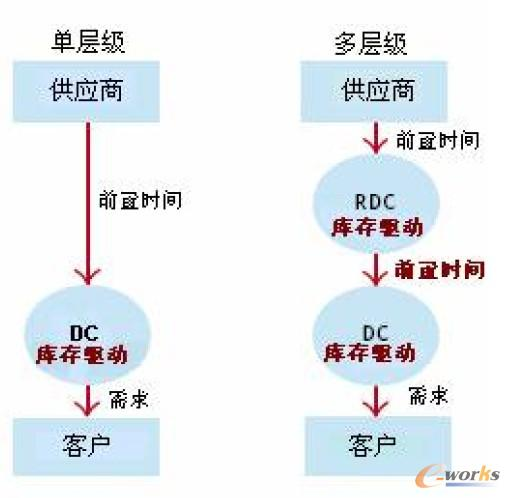
\includegraphics[scale=.6] {ml-info.jpg}
            \caption {库存驱动} \label {fig:mlinfo}
        \end{center}
    \end{figure}

    图 \ref{fig:mlinfo} 阐述了库存驱动因素怎样在两个层级中联系起来。循环节点代表了企业控制下的分销中心。标有“DC”的节点代表存储相同产品的所有DC。用红色标出的库存驱动因素是企业可以控制的。也就是说,补货周转率、订单供应战略和服务水平目标是补货控制变量,一个决策制定者能够影响装载的库存数量和提供给下端客户的服务水平。在单层级案例中决定控制变量的方法是众所周知的,但是你怎样才能在多层级案例中设置控制变量呢?今天,企业主要使用以下两种方法:

    \begin{enumerate}
        \item  将单层级方法应用到网络中的每个层级中。
        \item  使用配送需要计划(DRP)方法或者它的改进方法。
    \end{enumerate}

    \subsection { 多级库存的优化}

    常见的多级库存优化管理的方法有两种:顺序排列法和DRP法。

\subsubsection { 一、顺序排列法}

    这方法遵循了基本路线。在单层级案例中所采用的方法在多层级案例中实施了两次——一次在他们库存驱动因素的基础上对DC 进行了补货,然后在基于它的库存驱动因素的基础上向RDC 进行补货。在这个案例中,DC 利用了终端客户需求和RDC 前置时间。RDC 的前置时间是十分明显的;它们仅仅是对供应商而言的。但是怎么为RDC 进行需求预测呢?一种方法是将需求建立在从DC 到RDC 的历史订单基础之上。另一种方法是简单地传递来自DC 终端客户的需求。正如我们所看到的那样,这两种方法都是有缺陷的。

    \begin{figure}[bcth]
        \begin{center}
            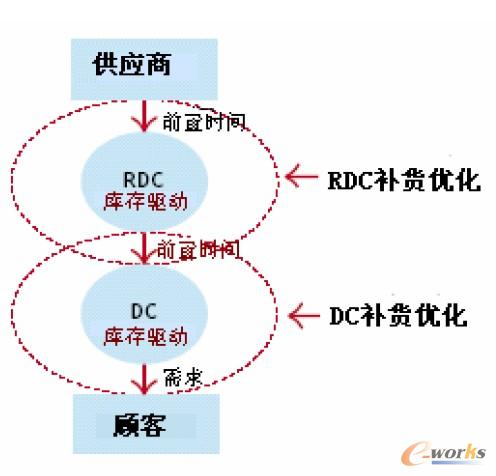
\includegraphics[scale=.6] {mlopt-1.jpg}
            \caption{顺序排列法} \label{fig:mlopt1}
        \end{center}
    \end{figure}

    图 \ref{fig:mlopt1} 说明了DC 和RDC 的补货方法,如前所述。这是一个顺序排列法,它将多级补货过程分成两个独立的阶段——一个阶段是为DC 补货,另一个阶段是为RDC 补货。但是这种方法带来了许多问题:

    \begin{enumerate}
        \item  缺乏需求链前向可视性

        当 DC 进行补货时,处于RDC 上游的供应商通常被遗忘。特别是DC 往往会忽视前置时间,当然除了来自RDC 的前置时间之外。而DC 一般也想当然地认为RDC 会在任何时间都能完全满足它的补货订单需求。最后,DC 对于RDC 的库存状况没有可视性。

        \item  缺乏需求链后向可视性

        当 RDC 进行补货时,通常会遗忘DC上游的客户。此外,RDC 对于DC 的库存状况货需求状况也没有可视性。

        \item  牛鞭效应带来的需求扭曲

        因为 RDC 和DC 有独立的需求预测(在基于他们各自直接的客户需求),牛鞭效应在RDC 和DC 之间造成了需求波动。这个结果导致RDC 不必要的库存。

        \item  整个网络成本难以评估

        当 RDC 或DC 的补货策略发生变化(如,通过改变可控库存驱动因素),新策略在另一级产生的隐含成本没有考虑进来。人们通常仅仅关注于对最近一级产生的影响。
    \end{enumerate}

\subsubsection { 二、配送需要计划法}

    配送需要计划(DRP)是材料供应计划(MRP)的拓展。制造商利用MRP 对零部件需求进行决策。用来制造产成品的零件或者部件是需求相关项目。正如MRP 那样,DRP 方法不管理生产组合不同阶段相关的需求,它对产品处于不同配送网络层级的需求进行管理。在某种意义上说,更高一层级中的产品需求取决于对相同产品低一级的需求。采用DRP 方法,DC 水平的需求预测首先被用来开拓整体产品需求。这些预测和安全库存需求、库存状态信息结合在一起,最终得出DC 的净需求。这是一种类似于MRP 综合图表的方法。通过弥补由RDC 到DC 前置时间产生的DC 净需求并且加总相应的时间周期,RDC 各阶段的时程化需求得到计算。RDC 利用这些上传的需求进行补货。DRP 方法也有些缺点。它首要的缺陷是上传需求和前置时间的非确定性。一个直接的结果是RDC 安全库存通常是在主观的方式下进行决策的。因为需求确定地上传至RDC,所以没有进行安全库存决策的严格性方法。这也是为什么使用这种补货方法的企业一般对RDC 安全库存量使用拇指规则;这种不科学的方法直接产生了多余的库存。由此,如果安全库存决策在一定程度上是不精确的,那也一点都不令人惊讶了。DRP 方法在制造领域中已经比较常用了,生产和运输成本通常也比库存成本更令人关注。正如顺序排列方法一样,DRP 不能拓展需求链前向的可视性,也缺乏对库存优化的整体网络性看法。

    特别需要指出的是,两层级的安全库存之间是没有任何联系的。因此,任何试图打破两层级之间的最佳平衡库存都是不可行的。

\subsubsection { 三、对顺序排列和DRP 方法的评价}

    顺序排列和 DRP 方法都会导致多余的库存,也没有对最终客户必要服务水平的改进。虽然每一层级可能获得合理的结果——来自它对整体问题的近视性看法——结果不一定是对整个网络最佳的解决方案。也就是说,DRC 和DC 的全部库存在追求最终客户服务目标方面没有达到最小化。

\subsubsection { 四、多层级网络中的牛鞭效应}

    对于牛鞭效应以及它扭曲需求信息已经谈过很多了。虽然牛鞭效应也可能在单层级解决方案中出现,但是它通常是企业所不能控制的。

    然而,在多层级网络中事实就不是这样了。在这些案例中,企业一定要考虑和管理牛鞭效应。牛鞭效应是在需求信号处理、订单计量、对价格波动和短缺博弈的反应过程中,由独立理性决策引起的。顺序排列方法通过在不同层级使用多独立需求预测而陷入了牛鞭效应之中。在低层级中订单计量引起层级之间额外的需求变化。最后,在顺序排列或DRP 方法中,缺乏需求供应链前向和后向的可视性能为实现客户服务目标而产生过多的库存积累。一个多层级网络提供正确测量牛鞭效应的机会,以此确定它的根源,减少或消除它对需求供应链绩效的影响。忽视这种机会也就意味着让牛鞭效应降低预测的准确性,增加库存,增加运作成本,降低客户服务水平。

\subsubsection { 五、真正的多层级方法}

    当一个有多层级网络的企业使用多层级方法管理库存时,主要的目的在于在所有的层级中最小化总库存,同时满足对最终客户的服务承诺。既使库存是主要的焦点,但是运输、仓储运作费用同样也在考虑之中,因为它们的成本因素也是优化的一部分。顺序排列和DRP方法将每个层级都看成是一个独立的问题,没有考虑到一个层级的库存可能对另一个层级可能产生较大的影响。采用多层级方法,需求预测和库存补货决策在单个优化过程中是在企业这个层面进行的。具体来说,真正的多层级方法应该是这样的:

    \begin{enumerate}
        \item  避免每个层级中的多头独立预测

        在 DC 的主要客户需求信号和其他信息驱动着所有层级的预测。真正的多层级方法消除了对于下游客户需求的依赖。

        \item  计算所有前置时间和前置时间的波动

        在每个层级上,补货决策计算了所有上游供应商而不仅仅是直接供应商的前置时间和前置时间的波动。

        \item  控制和管理牛鞭效应

        企业测算需求扭曲和确定可能采取的正确行动的根源。

        \item  实现需求链前向和后向的可视性

        每个层级利用其他层级库存位置的可视性——现有的、已定购尚未交货的、履行和延期交货的。在DC 层级,这意味着否定了对短缺博弈的任何需要。在RDC 层级,对DC 库存的可视性改进了需求的产生。

        \item  同步化订单策略

        将 DC 的订货周期与RDC 的运作实现同步化能减少RDC 和DC 之间的前置时间和前置时间波动。多层级模式能评估对不同同步化策略对两个层级的冲击。

        \item  提供差异化服务水平

        RDC 能为不同的DC 提供不同的服务水平(相同的产品)。一个多层级方法使之成为可能,因为企业控制一个产品在什么时间以什么方式进入或者离开RDC。

        \item  正确模拟一个层级替代性补货策略对另一个层级的交互式影响

        替代性策略包括不同补货周期、订单供应策略、服务水平目标和 SKU 层化。
    \end{enumerate}


\practices
\subsection{物料分类管理}
物料分类的模型图:
\screenshot{category.png}
某个物料分类可以0到多个子分类,子分类可以还有自己的子分类。

\subsubsection{物料分类设置}
在其中新增分类时,有一个“分类性质”,这个属性是在BOM模块中起作用的。只有在分类性质为成品或半成品下面的物料才能设置BOM
\opset{物料分类设置}{
    \item \ops{新建物料分类}{
        \item  点击工具单上的\button{新建}按钮,进入新建物料分类界面
            \screenshot{9.png}
        \item  选择上级分类
        \item  输入\textbox{分类名称}
        \item  选择分类性质
        \item  输入\textbox{分类描述}
        \item  点击\button{保存}按钮,保存新建的物料分类
    }
    \item \ops{查看物料分类}{
        \item  选择需要查看的物料分类
            \screenshot{11.png}
        \item  点击工具栏上的\button{查看}按钮,查看分类的详细信息
    }
    \item \ops{修改物料分类}{
        \item  选择需要修改的物料分类
        \item  点击工具栏上的\button{修改}按钮,进入编辑物料分类界面
        \item  修改相应的信息
        \item  点击\button{保存}按钮,保存更改后的物料分类
    }
    \item \ops{删除物料分类}{
        \item  选择需要删除的物料分类
        \item  点击工具栏上的\button{删除}按钮,在弹出的对话框中点击确定,删除物料分类
            \screenshot{10.png}
    }
}


\subsection{物料管理}
物料的模型图:
\screenshot{material.png}
    \ul {
    \item  物料属于某个物料分类
    \item  基准价格用于销售于参考报价用
    \item  单位换算表用于一个物料有多种计量单位的情况
    \item  自定义属性可以给物料添加更多的属性值
    \item  推荐库位可以指定物料的常用的存放在仓库中的库位
    \item  物料附件可以上传任何类型的文件,为物料提供技术图纸,详细文档说明等
    \item \opset{物料管理}{
        \item \ops{新建物料}{
            \item  点击工具条上的\button{新建}按钮,进入新建物料界面
                \screenshot{12.png}
            \item  选择\button{物料分类}
            \item  输入\textbox{物料名称}
            \item  选择\button{物料单位},输入\textbox{单位提示}
            \item  输入\textbox{条形码}
            \item  输入\textbox{规格型号}
            \item  输入\textbox{备注}
            \item  如果物料有其他属性需要输入,点击\button{自定义属性}标签
                \screenshot{13.png}
                \ul {
                \item  点击\button{添加}按钮,弹出自定义属性界面
                \item  输入\textbox{属性名称}
                \item 输入\textbox{属性值}
                \item  点击\button{确定}按钮,添加自定义属性
                }
            \item  点击\button{保存}按钮,保存新建的物料
        }
    \item \ops{查看物料信息}{
        \item  选择需要查看的物料
            \screenshot{20.png}
        \item  点击工具栏上的\button{查看}按钮,或者点击工具里面的\button{查看图标}
    }
    \item \ops{修改物料信息}{
        \item  选择需要修改的物料
        \item  点击工具栏上的\button{修改}按钮,进入修改物料信息界面
        \item  修改物料相关信息
        \item  点击\button{保存}按钮,保存更改后的物料信息
    }
    \item \ops{设置物料价格}{
        \item  点击\button{价格设置}图标,弹出物料价格设置对话框,增加物料最新报价
            \screenshot{14.png}
    }
    \item \ops{单位换算设置}{
        \item  点击\button{单位换算表设置}图标,弹出单位换算表设置对话框
            \screenshot{15.png}
        \item  点击\button{增加换算关系}按钮,弹出新增单位换算对话框
        \item  选择\button{目标单位}
        \item  输入\textbox{换算率}
        \item  点击\button{保存}完成新的换算关系添加
    }
    \item \ops{推荐库位设置}{
        \item  点击\button{推荐库位设置}图标,弹出推荐库位设置对话框
            \screenshot{16.png}
        \item  点击\button{增加推荐库位}按钮,弹出库位选择对话框,选择库位
        \item  点击\button{保存},完成新的推荐库位添加
    }
    \item \ops{设置仓库选项}{
        \item  点击\button{仓库选项设置}图标,弹出仓库设置对话框
            \screenshot{17.png}
        \item  选择\button{仓库},设置\button{安全库存}及\button{循环盘点周期}
        \item  点击\button{保存},完成仓库设置
    }
    \item \ops{设置物料附件}{
        \item  点击\button{物料附件设置}图标,弹出附件设置对话框
            \screenshot{18.png}
        \item  点击\button{选择文件}按钮,选择需要上传的物料附件
        \item  点击\button{上传}按钮,上传附件
    }
    \item \ops{删除物料}{
        \item  选择需要删除的物料
        \item  点击工具栏上的\button{删除}按钮,在弹出的对话框中点击\button{确定}按钮,删除相应的物料
            \screenshot{19.png}
    }
    \item \ops{检索物料}{
        \item  在左侧物料分类栏中直接选择物料分类,会显示该分类下的物料
        \item  点击右侧搜索边条,根据实际需要检索
    }
    }
}


\subsection{设置}

\subsubsection{仓库设置}
\opset{仓库设置}{
    \item \ops{新建仓库}{
        \item  点击工具栏上\button{新建}按钮,弹出新建仓库对话框
            \screenshot{1.png}
        \item  输入\textbox{名称}
        \item  输入\textbox{地址}
        \item  输入\textbox{电话}
        \item  选择仓库\button{负责人}
        \item  点击\button{保存}按钮,保存新建仓库
    }
    \item \ops{查看仓库}{
        \item  选择需要查看的仓库
        \item  点击工具栏上的\button{查看按钮}或者列表中的\button{查看工具},查看选择的仓库信息
    }
    \item \ops{修改仓库}{
        \item  选择需要修改的仓库
        \item  点击工具栏上的\button{修改}按钮,进入到修改仓库信息对话框
        \item  修改相应的信息
        \item  点击\button{保存}按钮,保存更改后的仓库信息
    }
    \item \ops{删除仓库}{
        \item  选择需要删除的仓库
        \item  点击工具栏上的\button{删除}按钮,在弹出的对话框中点击\button{确定},删除相应的仓库信息
            \screenshot{2.png}
    }
}

\subsubsection{库位设置}
\opset{库位设置}{
    \item \ops{新建库位}{
        \item  选择仓库
            \screenshot{7.png}
        \item  点击工具栏上的\button{新建}按钮,弹出新建库位对话框
            \ul {
            \item  在对话框中选择\textbox{上级库位}
            \item  输入\textbox{库位名称}
            \item  选择\button{库位容量单位}
            \item  输入\textbox{库位容量}
            \item  输入\textbox{容量单位提示}
            \item  输入\textbox{等级}
            }
        \item  点击\button{保存}按钮,保存新建的库位
    }
    \item \ops{查看库位}{
        \item  选择需要查看的库位
            \screenshot{6.png}
        \item  点击工具栏上的\button{查看}按钮,查看库位的详细信息
    }
    \item \ops{修改库位}{
        \item  选择需要修改的库位
        \item  点击工具栏上的\button{修改}按钮,进入库位修改对话框
        \item  修改相应内容
        \item  点击\button{保存}按钮,保存修改后的库位信息
    }
    \item \ops{删除库位} {
        \item  选择需要删除的库位
        \item  点击工具栏上的\button{删除}按钮
        \item  在弹出的确认对话框中点击\button{确定},删除相应的库位
            \screenshot{8.png}
    }
}


\subsection{日常业务}

\subsubsection{库存初始化}
\opset{库存初始化}{
    \item \ops{新建库存初始化条目}{
        \item  选择要初始化库存的仓库
        \item  点击工具栏上的\button{新建}按钮,进入库存初始化界面
            \screenshot{5.png}
        \item  输入\textbox{摘要}
        \item  输入\textbox{描述}
        \item  选择\button{对应公司}及\button{对应部门}
        \item  点击\button{添加}按钮,弹出库存初始化条目对话框
            \screenshot{3.png}
            \ul {
            \item  选择\button{对应物料}
            \item  输入\textbox{批号}
            \item  输入\textbox{编组}
            \item  输入\textbox{备注}
            \item  输入\textbox{数量}
            \item  输入\textbox{单价}
            \item  选择\button{有效期限}
            \item  选择\button{库位}
            \item  选择\button{状态}
            \item  点击\button{确定}按钮,添加一条库存初始化条目
            }
        \item  点击\button{保存}按钮,保存新建的库存初始化单据
    }
    \item \ops{修改库存初始化条目}{
        \item  选择需要修改的库存初始化条目
        \item  点击工具栏上的\button{修改}按钮,进入库存初始化单据修改界面
        \item  修改相应的内容
        \item  点击\button{保存}按钮,保存更改后的库存初始化单据
    }
    \item \ops{删除库存初始化条目}{
        \item  选择需要删除的库存初始化单据
        \item  点击工具栏上的\button{删除}按钮
        \item  在弹出的确认对话框中点击\button{确定},删除对应的库存初始化单据
            \screenshot{4.png}
    }
}

\subsubsection{物料出入库}
本系统对不同类型的入库,直接从菜单上进行区分。例如:采购入库,生产入库,委外入库,销售出库,生产出库,计划出库,委外出库等
点击相应的菜单,进入到不同类型的入库单管理界面
\opset{物料出入库}{
    \item \ops{新建出入库单}{
        \item 选择需要出入库的仓库,选择仓库后,会显示最新的出入库单据
            \screenshot{27.png}
            \screenshot{28.png}
        \item 点击工具栏上的\button{新建}按钮,进入新建出入库单界面
        \item 输入入库单\textbox{简要}
        \item 输入\textbox{描述信息}
        \item 点击按钮,弹出选择对应公司(供应商/客户)对话框
            \screenshot{29.png}
        \item 选择相应的公司,点击\button{确定}按钮完成选择
        \item 点击按钮,弹出选择对应公司下对应部门的对话框
            \screenshot{30.png}
        \item 如果已经在对应公司下设置了部门,选择部门,点击\button{确定}按钮完成选择
        \item 击\button{添加}按钮,弹出添加出入库项目对话框
            \screenshot{31.png}
        \item 点击按钮,弹出选择物料对话框
            \screenshot{32.png}
        \item 选择一个物料,点击\button{确定}按钮,完成物料选择
        \item 输入\textbox{批号}
        \item 输入\textbox{编组}
        \item 选择\button{有效期}
        \item 选择\button{库位}(如果仓库下已经建立了库位),点击按钮,弹出选择库位对话框
            \screenshot{33.png}
        \item 如果仓库下已经建立了库位,会列出所有库位供选择。点击\button{确定}按钮完成选择
        \item 输入\textbox{数量}
        \item 输入\textbox{单价}
        \item 选择\button{币种}
        \item 选择物料\button{状态}
        \item 填写\button{备注}信息
        \item 点击\button{确定}按钮,完成入库项目添加
        \item 点击\button{修改}按钮,弹出修改入库项目对话框
        \item 点击\button{移除}按钮,移除入库项目
        \item 点击\button{保存}按钮,完成入库单添加
    }
    \item \ops{修改出入库单}{
        \item  选择需要修改的出入库单
        \item  点击工具栏上的\button{修改}按钮,进入修改出入库单界面
        \item  过程类似于新建出入库单
    }
    \item \ops{查看出入库单} {}
    \item \ops{删除出入库单} {
        \item  选择要删除的出入库单
           \screenshot{34.png}
        \item  点击工具栏上的\button{删除}按钮,弹出确认删除对话框
        \item  点击\button{确定}按钮,完成删除。
    }
}

\subsubsection{库存调拨}
\opset{库存调拨}{
    \item \ops{新建库存调拨单}{
        \item  选择需要调拨的仓库,选择仓库后,会显示最新的调拨单据。
            \screenshot{27.png}
            \screenshot{35.png}
        \item  点击工具栏上的\button{新建}按钮,进入新建调拨单界面.
        \item  输入\textbox{作业简要}
        \item  输入\textbox{作业描述}
        \item  选择\button{目标仓库}
        \item  点击按钮,选择调拨\button{操作人员}
            \screenshot{36.png}
        \item  选择调拨人员,点击\button{确定}按钮,完成选择
        \item  点击\button{添加}按钮,弹出添加调拨项目对话框
            \screenshot{37.png}
        \item  点击按钮,弹出选择物料对话框
            \screenshot{38.png}
        \item  选择需要调拨的物料,点击\button{确定}按钮,完成选择
        \item  输入\textbox{批号}
        \item  输入\textbox{编组}
        \item  选择\button{有效期}
        \item  点击按钮,弹出库位选择对话框
            \screenshot{39.png}
        \item  点击\button{确定}按钮,完成库位选择
        \item  输入\textbox{数量}
        \item  输入\textbox{单价}
        \item  选择\button{币种}
        \item  选择\button{状态}
        \item  输入\textbox{备注}
        \item  点击\button{确定},完成调拨项目添加
        \item  点击\button{修改},修改调拨项目
        \item  点击\button{移除},移除调拨项目
        \item  点击\button{保存}按钮,完成碉堡单输入
    }
    \item \ops{修改库存调拨单}{
        \item  选择需要修改的库存调拨单
        \item  点击工具栏上的\button{修改}按钮,进入调拨单修改界面
        \item  修改过程类似新建库存调拨单
    }
    \item \ops{查看库存调拨单}{}
    \item \ops{删除库存调拨单}{
        \item  选择需要删除的\textbf{库存调拨单}
            \screenshot{43.png}
        \item  点击工具栏上的\button{删除}按钮,弹出确认删除对话框
        \item  点击\button{确定}按钮,完成删除
    }
}

\subsubsection{库存盘点}
\opset{库存盘点}{
    \item \ops{新建库存盘点表}{
        \item  选择需要盘点的仓库
            \screenshot{40.png}
        \item  点击\button{新建}按钮,新建库存盘点表
            \screenshot{41.png}
        \item  点击\button{查询}按钮,弹出物料查询对话框
            \screenshot{42.png}
        \item  点击\button{添加}按钮,弹出物料选择对话框
            \screenshot{23.png}
        \item  选择物料,点击\button{确定}按钮,完成选择
        \item  点击\button{移除},移除不需要盘点的物料
        \item  如果要盘点所有物料,勾选\textbf{所有物料}选项
        \item  点击\button{确定}按钮,把选择的物料添加到盘点表中
        \item  点击\button{查询}按钮,查询选择物料在仓库中的状态
        \item  盘点实际库存,和盘点表中的数据对比
        \item  选择物料,点击\button{修改}按钮,修改盘点项,录入盘点数据
        \item  选择物料,点击\button{移除}按钮,移除盘点项目
        \item  点击\button{保存}按钮,保存物料盘点表
    }
    \item \ops{修改库存盘点表}{
        \item  选择相应的库存盘点表
        \item  点击工具栏上的\button{修改}按钮,进入修改盘点表界面
        \item  修改相应的内容,过程类似于新建库存盘点表
    }
    \item \ops{查看库存盘点表}{}
    \item \ops{删除库存盘点表}{
        \item  选择需要删除的库存盘点表
        \item  点击工具栏上的\button{删除}按钮,弹出确认删除对话框
            \screenshot{43.png}
        \item  点击\button{确定}按钮,完成删除
    }
}


\subsection{查询}

\subsubsection{库存查询(含明细)}
库存查询,可以查询仓库的全部物料,也可以选择目标物料进行独立的查询。
\screenshot{21.png}
\ul {
    \item  选择需要查询的仓库
    \item  选择时间
    \item  点击查询按钮,弹出查询对话框,如下图
        \screenshot{22.png}
    \item  点击\button{添加}按钮,弹出选择物料对话框
    \item  点击\button{确定}按钮,选择需要查询的物料
    \item  点击\button{移除}按钮,移除不需要查询的物料
    \item  勾选\button{所有物料},本次查询即为查询仓库下所有物料
    \item  点击\button{查询}按钮,在查询结果表单中列出物料列表
        \screenshot{23.png}
        \screenshot{24.png}
    \item  点击\button{确定}按钮,完成物料查询,列出查询的物料
        \screenshot{25.png}
    \item  在操作列中点击\button{明细},弹出该物料的出入库详细信息
        \screenshot{26.png}
    \item  在出入库明细列表中,点击\button{所在},显示出入库所在单据以及所在仓库等详细信息
}
